\documentclass[10pt,a4paper]{scrartcl}
\usepackage[a4paper,vmargin={30mm},hmargin={30mm}]{geometry}
\usepackage[utf8x]{inputenc} % Unicode-Encoding
\usepackage[ngerman]{babel} % Neudeutsche Silbentrennung (mehrsprachiges Dok.)
\usepackage{ucs}
\usepackage{amsmath}
\usepackage{amsfonts}
\usepackage{amssymb}
\usepackage{parskip} % Skip indentation of first row
\usepackage{graphicx} % Graphics support
\usepackage{float} % Use H placement specifier for floats
\usepackage{longtable} % Tables across several pages
\usepackage{hyperref} % Hyperlinks
\usepackage{ccicons} % Creative commons
\author{Danilo Bargen, Jonas Furrer, Christian Fässler}
\title{Reptitionsfragen PnProg}
\input{revision}
\date{Version vom \revisiondate}

\begin{document}

\begin{titlepage}
	\maketitle
	\begin{center}\Huge\ccPublicDomain\end{center}

	\vspace{65mm}

	\subsubsection*{Über diese Zusammenfassung}

	Diese Sammlung an Repetitionsfragen wurde basierend auf dem Stoff des Herbstsemesters 2011 erstellt.
	Sie wird als gemeinfrei ({\ccPublicDomain} public domain) veröffentlicht - du kannst damit machen,
	was du willst. Höchstwahrscheinlich gibts darin jedoch noch viele Vertipper, Grammatikfehler und
	sonstige Unschönheiten. Wir bitten dich daher, an die zukünftigen Studenten zu denken, indem du
	diese Fehler notierst oder am besten gleich selber behebst.

	Desweiteren bitten wir dich, dass du deine eigenen überarbeiteten Versionen nicht selbstständig
	z.B.  auf dem Studentenportal veröffentlichst, sondern die Änderungen ins Originaldokument
	einpflegst, um einen Wildwuchs an Dokumentversionen zu vermeiden.

	Um Änderungen beizutragen, einfach auf Github einen Pull Request stellen (URL siehe unten).

	Das Dokument findest du an folgenden Orten:

	\begin{description}
		\item[Quellcode] https://github.com/HSR-Stud/PnProg
		\item[PDF-Version] http://studentenportal.ch/dokumente/pnprog/
	\end{description}

	Vielen Dank!

	\vspace{10mm}

	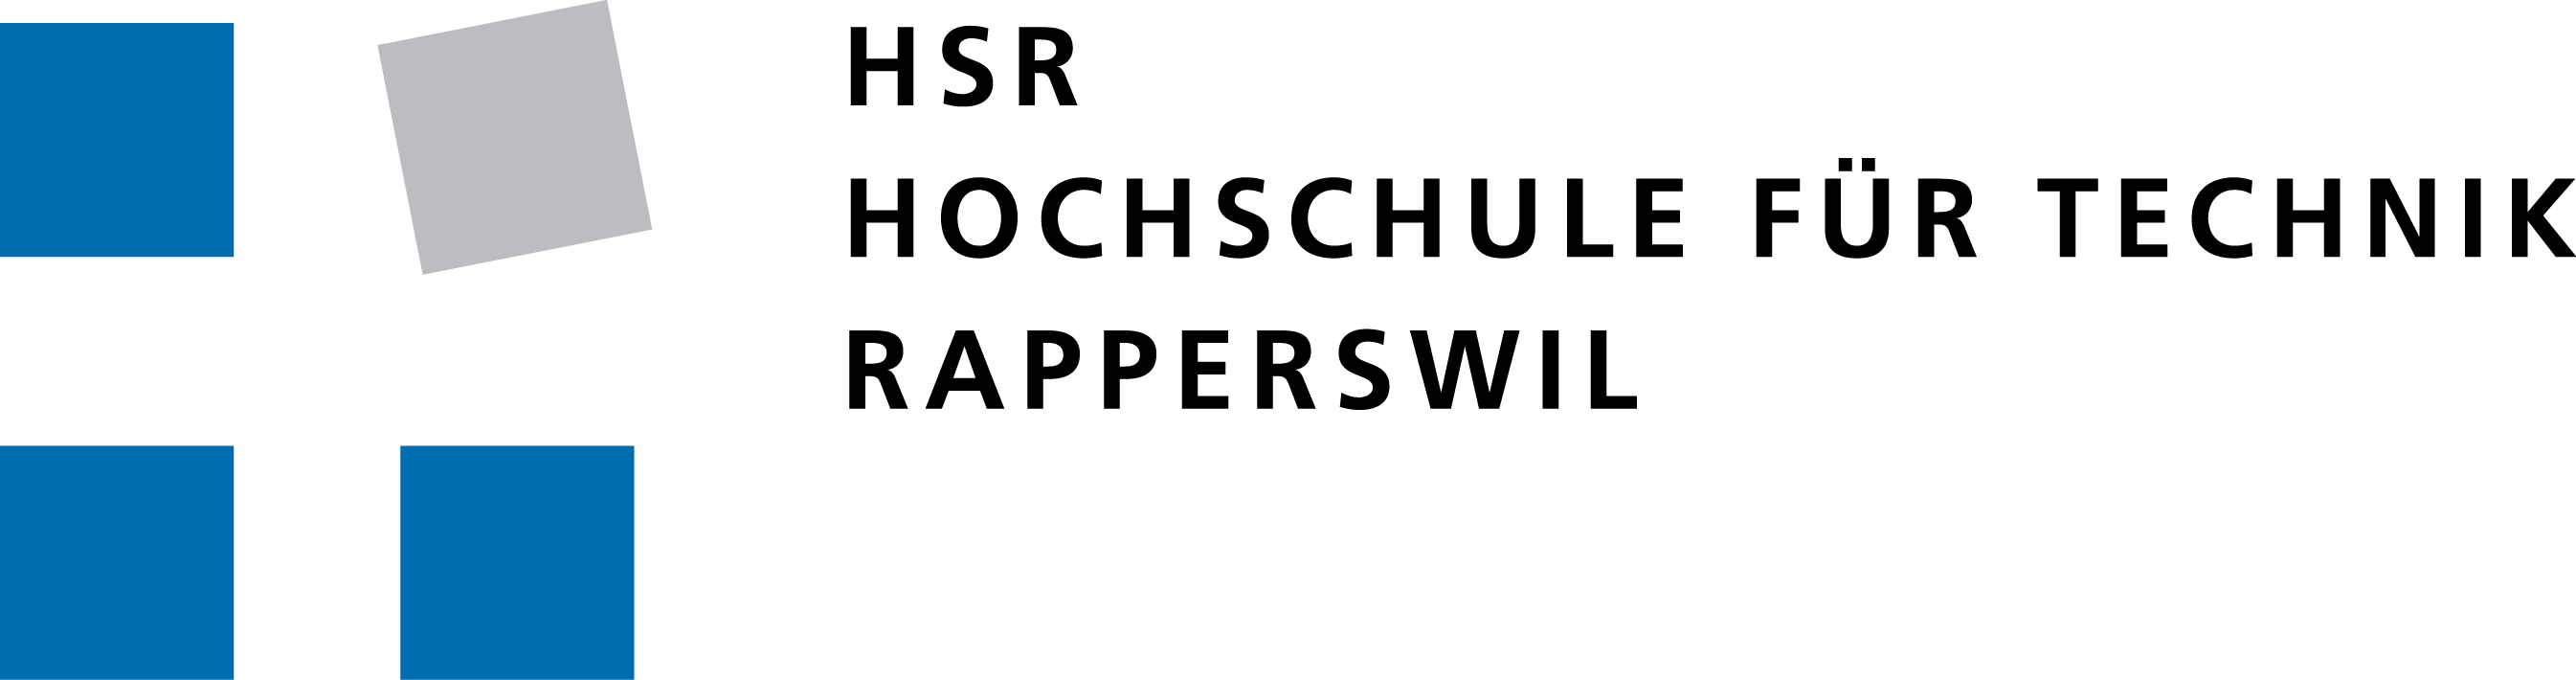
\includegraphics{hsr_logo.png}
	\thispagestyle{empty} % Don't start page numbers on this page
\end{titlepage}

\setcounter{secnumdepth}{0}
\tableofcontents

\newpage

\section{Woche 1}

\subsubsection{Was ist der Unterschied zwischen einem Prozess (Schwergewichtsprozess) und einem
Thread (Leichtgewichtsprozess)?}

\begin{itemize}
	\item Schwergewichtsprozess: Parallele Ausführung von Programmen, eigener Adressraum.
	\item Leichtgewichtsprozess: Parallele Ausführung innerhalb eines Prozesses, teilen Adressraum.
\end{itemize}

\subsubsection{Was ist Prozessor Multiplexing?}

Verzahnte Ausführung, Threads werden in Teilsequenzen ausgeführt. Illusion der Parallelität.
   
\subsubsection{Was bewirkt \texttt{yield()}?}

Wenn \texttt{yield()} auf einem Thread ausgeführt wird, gibt dieser den Prozessor frei, so dass ein
Anderer Thread ausgeführt werden kann. Der Thread bleibt allerdings im \textit{Ready-State} und wird beim
nächsten Schedulingzyklus wieder ausgeführt.

\subsubsection{Welche Zustände kann ein Thread haben (Thread Lifecycle)?}

Created, Alive, Terminated

\subsubsection{Wie kommt ein Thread in den Zustand "terminiert"?}

Ein Thread wird terminiert entweder durch den Aufruf von \texttt{stop()} auf dem Thread, oder wenn
die \texttt{run()} methode abgeschlossen ist (\texttt{run()} returns).
   
\subsubsection{Kann er nach Terminierung neu gestartet werden?}

Nein, ein beendeter Thread kann nicht neu gestartet werden.
   
\subsubsection{Was bewirkt \texttt{t.join()}?}

Der Aufruf von \texttt{join()} ist blockierend und wartet bis der Thread auf dem die Methode
aufgerufen wurde beendet ist. 
   
\subsubsection{Was passiert bei \texttt{Thread.currentThread().join()}?}

Dieser Aufruf blockiert das Programm vollständig (freeze); der Aufruf bewirkt, dass der aktuelle
Thread auf seine eigene Beendigung wartet und dadurch ewig läuft (Deadlock).
   
\subsubsection{Welche Art von Scheduling verwendet Java? Wie funktioniert es? }

Java verwendet \textit{preemtive priority based scheduling}. Dieser Scheduler nimmt immer ready Threads
mit höherer Priorität zuerst. Eine Änderung der Threadpriorität kann zu Blockierungen führen.


\section{Woche 2}


\subsubsection{Thread A wird 2x und B 1x gestartet (gleichzeitig). Was sind die möglichen
Ausgaben?}

\begin{verbatim}
Thread A:
    synchronized(v) { 
        System.out.println("A1"); 
        v.wait(); 
        System.out.println("A2"); 
    }   
Thread B:
    synchronized(v) {
        System.out.println("B1");
        v.notify();
        System.out.println("B2");
    }   
\end{verbatim}

(\texttt{v} referenziert dasselbe Objekt in allen Threads)

Mögliche Ausgaben:
\begin{itemize}
	\item \texttt{A1 A1 B1 B2 A2}
	\item \texttt{B1 B2 A1 A1}
	\item \texttt{A1 B1 B2 A2 A1}
	\item \texttt{A1 B1 B2 A1 A2}
\end{itemize}

Einschränkungen: \texttt{A2} kommt max. 1x, \texttt{B1} vor \texttt{A2}, \texttt{B1} und
\texttt{B2} zusammen.
  
\subsubsection{Welche zwei Synchronisationsarten unterscheidet man?}

Gegenseitiger Ausschluss (Mutual Exclusion) und Zustandssynchronisation.
  
\subsubsection{Was ist ein Kritischer Abschnitt?}

Codeabschnitt der nur von einem Thread zur gleichen Zeit ausgführt wird, keine verzahnte oder
parallele Ausführung innerhalb des Blockes. Wird erreicht durch gegenseitigen Auschluss (Mutual
Exclusion).
  
\subsubsection{Wann benutzt man \texttt{notify()} und wann \texttt{notifyAll()}?}

\begin{sloppypar}  % do line breaks before \texttt
\texttt{notify()} weckt einen beliebigen Thread wohingegen \texttt{notifyAll()} alle wartenden
Threads weckt. Im Normalfall kann immer prophylaktisch \texttt{notifyAll()} verwendet werden,
jedoch \textbf{muss} \texttt{notifyAll()} verwendet werden wenn mehrere Wartebedingungen
existieren, oder wenn die Möglichkeit besteht, dass nicht alle Threads die Bedingungen erfüllen
können. Zudem auch wenn es nicht gegeben ist, dass nach Erledigung immer notifiziert wird.
\end{sloppypar}
  
\subsubsection{Was ist ein "`Spurious Wakeup"'?}

Ein Thread kann auch "`aufwachen"' ohne ein Signal zu bekommen. Diese sogenannten "`Spurious
Wakeups"` können durch einzelne Betriebssysteme verursacht werden und sind nicht spezifiziert. Die
Folge daraus ist, dass man, wenn man Wartebedingungen definiert, mit unerwareten Threads rechnen
muss.
  
\subsubsection{Was ist Starvation?}

Wenn ein Thread aufgeweckt wird, muss er neu um den Monitor kämpfen. Es kann passieren, dass ein
Thread ständig überholt wird und nie mehr in den Monitor eintreten darf. (Kontinuierliche
Fortschrittsbehinderung eines Threads wegen Fairness-Problemen)
  
\subsubsection{Was ist der Unterschied zwischen einem Monitor-Lock und einem Monitor?}

Monitor-Lock != Monitor, jedes Java Objekt hat ein Monitor-Lock, aber nicht jedes Java Object ist
ein Monitor, ein Monitor wird implementiert durch \texttt{synchronized()}, \texttt{wait()},
\texttt{notify()}, \texttt{notifyAll()}.
  
\subsubsection{Auf welcher Ebene existieren Monitor-Locks (was kann locked werden)?}

\begin{sloppypar}  % do line breaks before \texttt
Jedes Objekt hat einen Lock. Es können Instanzen (\texttt{synchronized(obj)}) und Klassen
(\texttt{synchronized(Object.class)}) "`gelocked"' werden (nicht Methoden oder Variablen)
\end{sloppypar}
  
\subsubsection{Was ist das Problem bei geschachtelten oder rekursiven Locks?}

Rekursive und geschachtelte Locks sind potentiell Deadlock gefährdet.
  
\subsubsection{Wann wird ein Lock wieder freigegeben?}

Locks werden beim Verlassen des synchronized Blocks wieder freigegeben, auch wenn dieser durch eine
Exception verlassen wird.
  
\subsubsection{Was geschieht mit einem Lock, wenn innerhalb einen synchronized Abschnitt
\texttt{sleep()} oder \texttt{yield()} aufgerufen wird?}

Nichts besonderes, beide Methoden haben keinen Einfluss auf den Lock.
  
\subsubsection{Was passiert wenn \texttt{wait()}, \texttt{notify()} oder \texttt{notifyAll()}
ausserhalb eines synchronized Blocks aufgerufen werden?}

\texttt{IllegalMonitorStateException} (unchecked).


\section{Woche 3}

\subsubsection{Was sind die Bedingungen für das Auftreten von Deadlocks?}

\begin{itemize}
	\item Gegenseitige Sperren zwischen Threads
	\item Nested Locks innerhalb Thread
	\item Sperren ohne Timeouts oder Abbruchmöglichkeit
	\item Zyklische Warteabhängigkeiten
\end{itemize}
  
\subsubsection{Wie lassen sich Deadlocks vermeiden?}

Lineare Ordnung der Ressourcen einführen (Linearesperrordnung) oder grobgranulare Locks wählen.
(Oder Sequentielle Programmierung :D)

\subsubsection{Wie kann Starvation vemieden werden?}

FIFO Warteschlangen, möglich mit Semaphoren, Lock \& Condition und Read-Write Lock. Der Java
Monitor ist grundlätzlich unfair und somit starvationgefährdet.

\subsubsection{Welches sind die Korrektheitskriterien für Parallelität?}

\begin{itemize}
	\item Gegenseitiger Ausschluss: Kritsche Abschnitte auf gemeinsame Ressource sind
		synchronisiert
	\item Fortschritt: Niemand muss auf anderen Thread warten wenn er auf eine freie Resource
		zugreifen will
	\item Keine Deadlocks
	\item Keine Starvation
\end{itemize}

\subsubsection{Was ist eine Semaphore? Für was eignet sie sich?}

Synchronisationsprimitive. Abstrakter Datenyp mit Zähler. Mit Semaphoren kann gegenseitiger
Ausschluss realisiert werden. Semaphoren werden mit einer bestimmten Anzahl Ressourcen
initialisiert. Diese Ressourcen können dann angefordert werden (\texttt{acquire()}); falls keine
Resource mehr vorhanden ist wartet der Aufrufer. Ressourcen werden durch ein \texttt{release()}
wieder freigegeben, dieser Vorgang notifiziert die wartenden Threads.  

\begin{sloppypar} % enforce linebreak
Semaphoren werden auch in Betriebssystemen eingesetzt, wo sie interprozess-Synchronisation
ermöglichen.
\end{sloppypar}
  
\subsubsection{Welche Semaphore-Typen gibt es?}

\begin{itemize}
	\item Allgemeine Semaphore: Werte von $0$ bis $n$, für Quotas, Service Throttling, etc.
	\item Binary Semaphore: Werte $0$ oder $1$, für gegenseitigen Auschluss (Mutual Exclusion,
		\textit{Mutex}).
	\item Faire Semaphore: FIFO Warteschlange, default in Java ist unfair.
\end{itemize}
  
\subsubsection{Was sind Locks \& Conditions? Für was eignen sie sich?}

Synchronisationsprimitive. Kombination aus Lock für gegenseitigen Auschluss und Conditions für
Zustands-Synchronisation. Jede Condition gehört zu einem Lock, es sind mehere Conditions pro Lock
möglich.
  
\subsubsection{Was ist ein Read-Write Lock? Für was eignet er sich?}

Synchronisationsprimitive. Erlaubt parallele Lese-Zugriffe und gegenseitigen Auschluss für
Schreib-Zugriffe. Eignet sich besonders, falls viele Lese- und wenige Schreibzugriffe auf einem
Objekt erfolgen.


\section{Woche 4}

\subsubsection{Wie funktioniert ein Thread Pool?}

Ein Thread Pool besteht aus einer Task Queue und einem Thread/Worker Pool. Tasks implementieren
Arbeitspakete die parallel ausgeführt werden können. Die Worker-Threads holen sich Tasks aus der
Warteschlange und führen sie (parallel) aus.
  
\subsubsection{Was sind die Vorteile eins Thread Pools?}

Die Anzahl der Threads ist beschränkt. Keine Verlangsamung der Systems durch Überschreitung des
verfügbaren Speichers.

Threads können recycliert werden, Overhead für die Erzeugung der Threads wird eingespart.

Höhere Abstraktion, Trennung von Problem Space (Tasks) und System Space (Worker).

Individuelle Anpassung der Thread Anzahl pro System möglich (dadurch neuer "`Free Lunch"').
  
\subsubsection{Wann ist ein Thread Pool nicht geeignet?}

Die Tasks müssen relativ unabhängig von einander sein, ansonsten besteht Deadlock-Gefahr.
  
\subsubsection{Was ist der Unterschied zwischen "`Thread-Pool Executors"' und dem
"`Fork-Join-Pool"'?}

Thread-Pool Executors: seit Java 1.5, einfacher Thread-Pool, keine rekursiven Aufgaben.

Fork-Join-Pool: seit Java 1.7, unterstützt rekursive Aufgaben, benutzt "`Work-Stealing"' Verfahren.
  
\subsubsection{Was ist ein "`Future"'?}

Datentyp. Ein "`Future"' repräsentiert ein zukünftiges Resultat (Proxy auf Resultat). Kann
Berechnung auch abbrechen.
  
\subsubsection{Was sind typische Probleme eines Thread Pools?}

Warte-Abhängigkeiten zwischen Tasks - Deadlock-Gefahr.

Race Conditions - nicht synchronisierte Zugriffe auf gemeinsame Ressource von mehreren Tasks.

Über-Parallelisierung - Langsam wegen zu vielen kleinen Tasks. Der Schwellwert ist schwierig zu
bestimmen, oft nur durch den Programmierer.
  

\section{Woche 5}

\subsubsection{Was versteht man unter Cache-Kohärenz?}

Durch die Sicherstellung von Cache-Kohärenz wird bei Mehrprozessorsystemen mit mehreren CPU-Caches
verhindert, dass die einzelnen Caches für die gleiche Speicheradresse unterschiedliche
(inkonsistente) Daten zurückliefern. Änderungen im Cache eines Threads/CPU werden nicht direkt
in einem anderen Thread/CPU sichtbar. Reihenfolge der Änderungen kann unterschiedlich sein.
  
\subsubsection{Auf welche Variablen ist in Java der Zugriff atomar?}

\begin{itemize}
	\item Auf primitiven Datentypen (32 Bit), also ohne \texttt{long} und \texttt{double}
	\item Auf Objekt-Referenzen (egal ob 32 od. 64 Bit)
	\item Auf Variablen mit \texttt{volatile} Keyword (\texttt{long} und \texttt{double} mit
		\texttt{volatile} sind auch atomar)
\end{itemize}
  
\subsubsection{Kann man Unteilbarkeit (atomarität) und Sichtbarkeit gleichsetzen?}

Nein, Atomarität bewirkt keine Cache-Kohärenz, ein Thread sieht nach dem Schreiben evtl. noch einen
alten Wert, jedoch ist der Wert immer gültig.
  
\subsubsection{Was bewirkt eine Deklaration mit dem Keyword \texttt{volatile}?}

\begin{itemize}
	\item Atomaren Schreib- und Lesezugriff für \texttt{long} und \texttt{double}.
	\item Lese- und Schreibzugriff invalidieren Cache-Line.
	\item Keine Optimierung oder Umsortierung durch Compiler/CPU (über die Grenzen von
		\texttt{volatile} Zugriffen)
	\item Vergleichbar mit \texttt{synchronized} Getter/Setter, jedoch effizienter, da nicht blockiert
		wird.
\end{itemize}
  
\subsubsection{In welchen Fällen garantiert Java die Sichtbarkeit?}

\begin{itemize}
	\item Release eines Locks aktualisiert den Hauptspeicher (Cache Flush)
	\item Acquire eines Locks lädt Variablen neu aus dem Hauptspeicher (Cache Flush)
	\item \texttt{volatile} Variable, schreiben aktualisiert Hauptspeicher (Cache Flush)
	\item \texttt{volatile} Variable, lesen lädt neu aus dem Hauptspeicher (Cache Flush)
	\item Bei Thread-Start und -Ende wird der Hauptspeicher aktualisiert (Cache Flush)
	\item Initialisierung von \texttt{final} Variablen. Bei Zuweisung in Konstruktor sehen andere
		Threads den endgültigen \texttt{final} Wert, kein anderer Thread darf während Konstruktion
		zugreifen, bei nicht \texttt{final} Variablen ist der default Wert der Variable zu sehen.
\end{itemize}
  
\subsubsection{Welche Zusicherungen und Möglichkeiten bieten Java Atomic Variablen?}

\begin{itemize}
	\item Atomare Operationen, nicht nur Lesen und Schreiben.
	\item Benötigen kein Blockieren oder Warten.
	\item Effizient durch Verwendung von atomaren Instruktionen des Prozessors.
\end{itemize}
  
\subsubsection{Was versteht man unter "`as-if-serial"' Semantik?}

"`As-if-serial"' Semantik heisst, dass alle Optimierungen und Umsortierungen keine Folgen für das
serielle Model haben, d.h das Programm wird seriell vor und nach der Optimierung das selbe Resultat
liefern. "`As-if-serial"' gilt innerhalb von Threads. 
  
\subsubsection{Was versteht man unter optimistischer Synchronisation?}

Schreibe Änderung nur, sofern kein anderer Thread zwischenzeitlich geschrieben hat, ansonsten mit
dem neuen Wert wiederholen (Starvation-Gefahr). Dieses Vorgehen wird durch atomare Variablen
ermöglicht:
    
\begin{verbatim}
do {
    int oldValue = var.get();
    int newValue = calculateChanges(var);
    success = var.compareAndSet(oldValue, newValue);
} while (!success);
\end{verbatim}
    
\subsubsection{Worin liegt der Vorteil wenn man Synchronisation verhindert?}

Ein Programm ohne Synchronisation ist grundsätzlich effizienter, weil nicht blockiert oder gewartet
wird (Synchronisation ist teuer). Zudem werden Deadlocks verhindert. 
  
\subsubsection{Wie kann Synchronisation verhindert werden?}

\begin{itemize}
	\item Verwendung von Read-Only Variablen, schreiben bevor verschiedene Threads zugreifen
		(\texttt{final}).
	\item Lokale Werte pro Thread, Stack, Instanzvariable des Thread, Java
		\texttt{ThreadLocal}.
\end{itemize}
  
\subsubsection{Was ist die \texttt{ThreadLocal} Klasse?}

Eine Klasse die es ermöglicht, Variablen als Klassenvariablen für jeden einzelnen Thread zu halten.
(Map mit ThreadID als Key)
  
\subsubsection{Welche der folgenden Vorgänge sind Atomar?}

\begin{tabular}{l l}
	\texttt{long l = -1;} & nicht atomar, Initalisierung und Zuweisung \\
	\texttt{double d = 3.14;} & nicht atomar, Initalisierung und Zuweisung \\
	\texttt{int i = 1;} & nicht atomar, Initalisierung und Zuweisung \\
	\texttt{String s = \dq first\dq;} & nicht atomar, Initalisierung und Zuweisung \\
	\texttt{boolean b = true;} & nicht atomar, Initalisierung und Zuweisung \\
	\texttt{i = (int)l; } & nicht atomar, Lesen eines 64 Bit Datentyp \\
	\texttt{l = 42; } & nicht atomar, 64 Bit Datentyp \\
	\texttt{i = 7;} & atomar \\
	\texttt{++i;} & nicht atomar, Lesen und Schreiben \\
	\texttt{s = \dq second\dq; } & atomar \\
	\texttt{d = d * i;} & nicht atomar, Lesen und Schreiben \\
	\texttt{s = null;} & atomar \\
	\texttt{b = false;} & atomar \\
\end{tabular}

Atomar ist alles was nur eine Aktion beinhaltet, exklusive \texttt{long} \& \texttt{double}, die
sind ohne \texttt{volatile} nie atomar, und exklusive Java Atomic Klassen.


\section{Woche 6}

\subsubsection{Welche zwei Grundkonzepte zur Vermeidung der Synchronisation gibt es?}

\begin{itemize}
	\item Immutability (Unveränderlichkeit)
	\item Confinement (Einsperrung)
\end{itemize}
  
\subsubsection{Wie kann man erreichen das ein Objekt ein Immutable Object ist?}

\begin{itemize}
	\item Alle Instanzvariablen als \texttt{private final} deklarieren. Verweis nur auf primitive
		Datentypen oder Referenzen auf wiederum Immutable Objects.
	\item Keine ändernden Methoden. Methoden können neue Objekte zurück liefern.
	\item Konstruktor initialisiert die Instanzvariablen. Kein Thread in Konstruktor starten der schon
		auf \texttt{this} oder Instanzvariablen zugreift.
	\item \texttt{equals()} nicht anhand der Referenz.
\end{itemize}
  
\subsubsection{Welche Klassen sind Beispiele für Immutable Objects aus dem \texttt{java.lang} Package?}

\texttt{java.lang.String} oder \texttt{java.lang.Integer}.
  
\subsubsection{Was ist Confinement und wozu dient es? }

Struktur garantiert, dass auf ein Objekt nur durch einen Thread zur gleichen Zeit zugegriffen wird.
Das Resultat ist, dass dieses Objekt nicht synchronisiert werden muss.
  
\subsubsection{Welche Arten von 'Confinement' gibt es?}

\begin{itemize}
	\item Method Confinement: Objekt wird nur in lokalen Variablen in einem Thread verwendet.
	\item Thread Confinement: Objekt ist nur über Referenzen von einem Thread erreichbar.
	\item Object Confinement: Objekt ist in einem anderen bereits synchronisiertem Objekt gekapselt.
	\item Group Confinement: Objekt wird zwischen Threads ausgetauscht, wobei jeweils immer nur ein Thread das Objekt besitzt.
\end{itemize}
  
\subsubsection{Was ist ein Hand-Off Protokoll?}

Unter Hand-Off versteht man die Übergabe eines Objektes von einem Thread an einen anderen Thread.
Dadurch wird sichergestellt, dass nur ein Thread das Objekt zur gleichen Zeit benutzt.
Üblicherweise wird das Objekt durch einen Tail-Call (= Übergabe als letzte Instruktion einer
Methode) weiter gegeben. Alternativen dazu sind Caller-Copies, Reciever-Copies, Werteparameter,
oder Trust (Empfänger ist verpflichet das Objekt nicht zu verändern oder weiter zu geben).
  
\subsubsection{Welche drei Konzepte helfen die Synchronisation zu reduzieren?}

\begin{itemize}
	\item Grobgranulare Locks: Pauschaler Lock für mehrere Objekte, ergibt weniger Locks, dafür auch
		weniger Parellelität.
	\item Thread-lokale Pools: Daten werden Thread-lokal zwischengelagert und nur sporadisch
		abgeglichen, Synchronisation ist nur bei globalen Ablgeichen nötig.
	\item Lock-freie thread-safe Strukturen: Atomare Operationen und \texttt{volatile} Keyword;
		Minimale Synchronisation auf Speicherebene.
\end{itemize}
  
\subsubsection{In welche Locking Kategorien kann man Objekte unterteilen?}
 
\begin{itemize}
	\item Non-shared: Auf dem Stack, Confinement, nicht zwischen Thread austauschbar $\rightarrow$ keine Synchronisation nötig.
	\item Read-only-shared: Zwischen Threads nutzbar aber keine Änderungen erlaubt $\rightarrow$ keine Synchronisation nötig.
	\item Shared: Mehrere Threads greifen gleichzeitig zu, Änderungen erlaubt $\rightarrow$ Synchronisation nötig.
\end{itemize}

\subsubsection{Sind die Java Collections thread-safe? Warum?}

Klassische (alte) Java Collections (\texttt{Vector}, \texttt{HashTable}) sind thread-safe.

Moderene Java Collections (\texttt{HashSet}, \texttt{ArrayList}, \texttt{LinkedList}, etc.) sind
nicht thread-safe.

Ganz neue Concurrent Collections (\texttt{ConcurrentHashmap}, \texttt{ConcurrentLinkedQueue},
\texttt{CopyOnWriteArrayList}, etc.) sind thread-safe. 

Warum: Synchronisation ist oft nicht nötig bei Thread-lokaler Verwendung (Confinement),
Synchronisationskosten sind unnötig hoch. Auch mit nebenläufigen Zugriffen sind thread-safe
Collections meist ungenügend da weder die Elemente noch die Iteration synchronisiert ist.
  
\subsubsection{Wie kann man nicht thread-safe Collections doch in einer multi-threading Umgebung nutzen?}

Clientseitige Synchronisation oder Verwendung von synchronized Wrappers.

\subsubsection{Was ist das Problem bei der Iteration mit Nebenläufigkeit?}

Ein anderer Thread kann parallel die Collection verändern. Bei Synchronisierten Collections sind
die Einzelzugriffe zwar synchronisiert, jedoch nicht die ganze Sequenz der Traversion.
  
\subsubsection{Welche Strategien gibt es für die nebenläufige Iteration?}

\begin{itemize}
	\item Fail-Fast Iteratoren: Bei Änderung der Collection Exception werfen.
	\item Snapshot Iteratoren: Kopie der Collection machen und darüber iterieren (evtl. grosser
		Speicher- und Kopieraufwand).
	\item Client-Side Locking: Deadlock-Gefahr.
	\item Enumeration Method Pattern: Collection implementiert die Iteration mit einem Strategie
		Object (Visitor), die Iteration ist synchronized innerhalb des Collection-Objects (nicht
		implementiert von Java Collections).
\end{itemize}


\section{Woche 7}

\subsubsection{Wo liegen die Unterschiede in der Struktur des Lockings von \texttt{synchronized}
Blocks und Lock-Primitiven?}

\texttt{synchronized} ist an ein Statement- oder Methodenblock gebunden.

Lock-Primitiven müssen immer paarweise aufgerufen werden (lock-unlock, acquire-release).

Synchronized Lock wird immer aufgehoben nach verlassen des Blocks, auch bei Exception,
Lock-Primitiven nicht (darum Lock-Freigabe immer in \texttt{finally} definieren).
  
\subsubsection{Was sind Gründe das Before-After Pattern zu verwenden?}

Durch die Verwendung dieses Pattern ist es möglich die Sperre und die Sperrfreigabe zentral zu
definieren und es muss jeweils nur noch die Kernfunktion der Klasse implementiert werden (Reusablity).
  
\subsubsection{Welche Implementationsmöglichkeiten gibt es für das Before-After Pattern?}

\begin{itemize}
	\item Vererbung
	\item Object Adapter
	\item Decorator
	\item Template Method
	\item Dynamischer Proxy
	\item Aspekt-Orientierung
\end{itemize}
  
\subsubsection{Was ist Strategized Locking?}

Trennung von Kernlogik und Locking. Daraus ergibt sich die Möglichkeit dieselbe Klasse mit oder
ohne Lock einzusetzen. Es können verschiedene Locking-Mechanismen bei der selben Klasse angewendet
werden.
  
\subsubsection{Wie kann man Strategized Locking umsetzen?}

Generisches Interface für Synchronisation (\texttt{void aquire()}, \texttt{void release()}) und
spezifische Implementierung des Interfaces. Für kein Locking leere Implementierung (Null-Objekt-Pattern).
  
\subsubsection{Für was sind Concurrency Design Patterns?}

Design Patterns für nebenläufige Modellierung, Fokus auf Threads und deren Interaktion.
  
\subsubsection{Welche Concurrency Design Pattens gibt es?}

\begin{itemize}
	\item Producer-Consumer, asynchrone Erzeugung und Weiterverarbeitung von Daten.
	\item Pipeline, Serie von nebenläufigen Verarbeitungsschritten.
	\item Divide and Parallel Conquer, Zerlegung in unabhängige parallel bearbeitbare Teilaufgaben.
\end{itemize}
  
\subsubsection{Was ist das Thread-Model von AWT/Swing/SWT?}

Alle genannten GUI-Frameworks nutzen das Single-Threading Modell. Sie nutzen einen Event Dispatch
Thread, ein Loop zur Ausführung der Ereignisse aus einer Event Queue.
  
\subsubsection{Wie sollen Threads mit dem GUI interagieren?}

Andere Threads müssen sich in der Event Queue einreihen. (Bsp. \texttt{SwingUtilities.invokeLater(Runnable)})
  
\subsubsection{Warum verwenden diese GUIs dieses Thread-Model?}

Synchronisationskosten, Locking aller Komponenten und Methoden wäre relativ teuer.
Hohes Deadlock-Risiko, oft zyklisch geschachtelte Aufrufe (MVC).
   
\subsubsection{Was sind die Einschränkungen davon?}

\begin{itemize}
	\item Keine langen Operation in Event Listener, diese würden das ganze UI blockieren.
	\item Keinen Zugriff auf UI Komponenten, dies würde zu Race-Conditions führen.
\end{itemize}


\section{Woche 8}

\subsubsection{Was ist ein Synchronisationspunkt?}

Ein Punkt in der Thread-Ausführung an dem eine Anzahl Threads auf eine gewisse Bedingung wartet,
nach der Erfüllung dieser Bedingung setzen alle Threads ihre Abarbeitung fort.
  
\subsubsection{Was sind Beispiele für Synchronisationspunkte?}

\begin{itemize}
	\item Parallele Rechnungen, warten auf Teilergebnisse um weiter zu rechenen.
	\item Rennspielsimulation
\end{itemize}
  
\subsubsection{Warum genügt \texttt{Thread.join()} nicht um Synchronisationspunkte umzusetzen?}

Nur ein Thread kann auf die Beendigung von anderen Threads warten. Die anderen Threads sind danach
beendet und können nicht wiederverwendet werden.
  
\subsubsection{Was sind Latches? }

Synchronisationsstruktur mit Zähler (ähnlich Semaphore), Threads warten bis Zähler \texttt{<=} 0 wird.
Ein Latch synchronisiert ein oder mehrere Threads auf eine Anzahl Ereignisse, ein Ereignis
entspricht einer Countdown Operation, synchronisiert wird bis der Zähler \texttt{<=} 0 ist.

In Java: \texttt{CountdownLatch}. Warten mit \texttt{await()} und Zähler reduzieren mit
\texttt{countDown()}. Da \texttt{countDown()} nicht blockiert, können Ereignisse durch beliebige
Threads an beliebiger Stelle ausgelöst werden.

Ein Latch ist nur einmalig verwendbar.
  
\subsubsection{Was sind Barriers?}

Synchronisationspunkt für bestimmte Anzahl Threads, erst wenn alle Threads den Punkt erreicht haben
können alle weitermachen.

In Java: \texttt{CyclicBarrier}. Warten mit \texttt{await()}. Anzahl Threads muss vorgegeben sein
wenn so viele Threads warten wird die Barrier aufgehoben.

Eine Barrier ist beliebig oft verwendbar. Sie wird beim Aufheben der Blockierung automatisch
resetted, oder kann manuell zurückgesetzt werden.
  
\subsubsection{Wie lassen sich Synchronisationspunkte sonst noch Umsetzen?}

z.B durch Semaphore oder auch Monitor.
  
\subsubsection{Was ist ein Rendezvous?}

Eine Barriere mit nur 2 Threads, die beim aufeinandertreffen Informationen austauschen.
In Java implementiert durch \texttt{Exchanger}.
  
\subsubsection{Wie kann man Daten zwischen Threads austauschen?}

\begin{itemize}
	\item Exchanger (Rendezvous): Spezialfall für zwei Threads. Synchrone Übergabe durch warten auf
		den Partner-Thread.
	\item Blocking Queue (Bounded Buffer): Producer/Sender legen Daten in Queue, Consumer/Empfänger
		entnehmen Daten aus Queue. Asynchrone Übergabe möglich, ausser Queue voll oder leer, daruch wird
		die Geschwindigkeit entkoppelt.
\end{itemize}
  
\subsubsection{Was sind asynchrone Aufrufe?}

Asynchrone Ausführung von (unter Umständen langlaufenden) Operationen, Caller kann dabei
weiterarbeiten. Die asynchrone Operation wird in einem seperaten Thread erledigt (z.B Task in
Thread Pool). Auf das Resultat der asynchronen Operation kann mittels Future Objekt oder Completion
Callback zugegriffen werden.
  
\subsubsection{Was sind \texttt{Future}-Objekte und Completion Callbacks? Wofür verwendet man sie?}

Future Objekte repräsentieren ein zukünftiges Resultat einer asynchronen Operation. Der Aufrufer
wird blockiert wenn er das Ergebnis abholen will bevor dieses vorliegt. Es ist möglich abzufragen
ob das Ergebnis schon vorliegt. Dies ist ein Caller-zentrischer Ansatz, der Caller synchronisiert
sich selbst auf die Beendigung der asynchronen Operation.

Completion Callback heisst, der Aufrufer definiert eine Callback-Methode die von der asynchronen
Operation aufgerufen wird wenn diese fertig ist. Dies ist ein Callee-zentrischer Ansatz, die
aufgerufene asynchrone Operation ruft zurück wenn sie fertig ist. Da die Callback-Methode von einem
anderen Thread aufgerufen wird ist evtl. Synchronisation zwischen den Zugriffen des Aufrufers und
der Callback-Methode nötig.
  

\section{Woche 9}
 
\subsubsection{Was sind die Hauptunterschiede zwischen TCP und UPD?}

\begin{itemize}
	\item TCP: Verbindungsorientiert, zuverlässiger Byte Strom zwischen zwei Punkten, kein Byte geht
		verloren.
	\item UDP: Nachrichtenorientiert, zustands- und verbindungslos, unzverlässig, Nachrichten können
		verloren gehen, dafür schneller als TCP (dank weniger Overhead), mehrere Empfänger adressierbar
		(Multicast).
\end{itemize}
  
\subsubsection{Welche Port-Bereiche gibt es?}

\begin{itemize}
	\item Well-known Ports: Socket-Bindung braucht Superuser-Rechte (0-1023).
	\item Registered Ports: Können von Applikationen benutzt werden, manche sind offiziell registriert
		(1024-49151).
	\item Ephemeral Ports: Werden vom Betriebssystem vergeben (49152-65535).
\end{itemize}
  
\subsubsection{Wieviele Anwendungen können den selben Port binden?}

Im Normalfall gilt eine Anwendung pro Port, Ausnahmen sind Multicast Sockets und die Verwendung der
Option \texttt{SO\_REUSEADDR} (\texttt{serverSocket.setReuseAddress(true)}).
 
\subsubsection{Was ist ein Socket?}

Ein Socket ist der Endpunkt einer Zweiwege-Kommunikation von zwei Prozessen über das Netzwerk.

Ein Socket ist an einen Port seines Hosts gebunden, daduch kann er eindeutig identifiziert werden.

Man unterscheidet Server Sockets und Client Sockets.
 
\subsubsection{Welche Informationen hat eine Socket-Adresse?}

Die Socket-Adress beinhaltet die IP-Adresse (v4/v6) und den Port, falls ein DNS-Name 
existiert, ist auch dieser enthalten.
 
\subsubsection{Welche Schritte braucht es, um den Server zu kontaktieren?}

Socket kreieren. In Java wird ein kombiniertes "`Create
and Connect"' durchgeführt. Wenn kein \texttt{bind()} verwendet wird, wird automatisch ein freier
Ephemeral Client-Port verwendet.

\texttt{new Socket(\dq addr\dq, port)}
 
\subsubsection{Wie werden mittels Java Sockets nach dem Verbindungsaufbau Daten ausgetauscht?}

Sockets haben einen Input- und Output-Stream. Der Read auf dem Inputsream blockiert bis Daten
angekommen sind (Timeout möglich). Die Daten werden als Byte-Stream übertragen. Mittels
\texttt{flush()} kann die Übertragung des Buffers erzwungen werden.
 
\subsubsection{Wie kann man in Java eine SSL Verbindung aufbauen? }

SSL-Verbindungen werden mittels einer Factory aufgebaut. Die Factory liefert einen SSLSocket.

\texttt{Socket socket = SSLSocketFactory.getDefault().createSocket()}.


\section{Woche 10}

\subsubsection{Welche Schritte sind für den Verbindungsaufbau auf der Serverseite nötig?}

\begin{itemize}
	\item Socket erzeugen.
	\item Bind (optional, Java macht kombiniertes Create and Bind). Potenzielle Fehler beim
		binden sind, dass der Socket bereits gebunden ist (\texttt{BindeException}) oder dass der Port
		bereits belegt ist (\texttt{IOException}).
	\item Listen. Erlaubt eingehende Verbindungen, passiert implizit durch den \texttt{accept()}.
	\item Accept. Wartet und akzeptiert eine eingehende Verbindung. Accept liefert eine neue Client
		Socket Instanz. \texttt{accept()} wird oft in einer Schleife aufgerufen um mehrere Verbindungen
		zu akzeptieren.
\end{itemize}

\subsubsection{Wie kann man einen Server an mehrere Adressen binden?}

Falls ein Server mehrere Adressen hat, kann er einen Socket an alle Adressen binden, dafür
verwendet er eine sogenannten \textit{Wildcard-Bind}: \texttt{bind(new InetSocketAddress(4321))} oder
\texttt{null} für die Adresse einsetzen.
  
\subsubsection{Was ist das Backlog?}

Das Backlog ist die Queue für wartende eingehende Verbindungen. Wenn die Queue voll ist, werden
\texttt{connect()} Abfragen abgewiesen. Gesetzt werden kann die Backlog Grösse im Konstruktor des
Sockets oder beim Binden. Default Backlog Grösse ist System abhängig, moderner Default ist ca. 128. 
  
\subsubsection{Was passiert wenn der Server \texttt{accept()} aufruft?}

Der Server wartet blockierend solange bis ein Client \texttt{connect()} aufruft. Beim Aufbau einer
Verbindung erhält der Server einen Client Socket als Resultat.
  
\subsubsection{Wie lassen sich mehrere Klienten durch einen Socket Server bedienen? }

\begin{itemize}
	\item Serieller Server (Single-Connection Server), nimmt jeweils eine Verbindung an und
		verarbeitet sie vollständig. Kommunikation mit nur einem Client auf einmal. (Backlog)
	\item Paraller Server (Multi-Connection Server), nimmt Verbindungen nacheinander an und
		verarbeitet sie parallel. 
\end{itemize}
  
\subsubsection{Welche Arten von parallen Servern gibt es? }

\begin{itemize}
	\item Multi-Threaded Server, nach \texttt{accept()} wird ein separater Thread für die
		Kommunikation benutzt.
	\item Multi-Prozess Server, nach \texttt{accept()} wird ein separater Betriebsystem-Prozess für
		die Kommunikation benutzt, dieses Vorgehen ist mit Java nicht möglich (\texttt{fork()} in C).
	\item Reactor Pattern, I/O Multiplexer, mehrere Anfragen gemischt in einem Thread verarbeiten.
\end{itemize}

\subsubsection{Was sind die Einschränkungen von Multi-Threaded Server?}

\begin{itemize}
	\item \texttt{java.net} Klassen sind nicht thread-safe
	\item Socket Instanzen dürfen nicht von mehreren Threads gleichzeitig zugegriffen werden
	\item \texttt{accept()} darf nicht von mehrern Threads gleichzeitig aufgerufen werden
	\item Backlog Grösse nur einmal bestimmbar (bei der Instanzierung des \texttt{ServerSocket} oder
		beim \texttt{bind()}).
\end{itemize}

\subsubsection{Wie erkennt der Server die IP-Adresse und Port des verbundenen Clienten?}

\texttt{accept()} auf der Serverseite liefert eine Instanz von einem Client Socket, darauf kann
mittels \texttt{Socket.getPort()} und \texttt{Socket.getInetAddress()} Adresse und Port der
Gegenseite herausfinden. Die eigenen Adresse und Port findet man mit den entsprechenden Aufrufen
von \texttt{Socket.getLocalPort()} und \texttt{Socket.getLocalAddress()}.
  
\subsubsection{Wie lassen sich in Java die IP-Adressen eines Domain Namens bestimmen?}

Die Klasse \texttt{InetAddress} bietet die statische Methode \texttt{getByName()} und
\texttt{getByAddress()} sowie die Instanzmethode \texttt{getHostName()}.

\begin{verbatim}
InetAddress address = InetAddress.getByName("152.96.37.60");
System.out.println(address.getHostName());
\end{verbatim}


\section{Woche 11}

\subsubsection{Welche I/O Modelle für Sockets gibt es?}

\begin{itemize}
	\item Blocking I/O, jeder Socket-Aufruf blockiert bis er fertig ist.
	\item Non-blocking I/O mit Polling, wiederholend auf Daten prüfen.
	\item I/O Multiplexing, ein Thread bearbeitet gemischt verschiedene Anfragen.
	\item Asynchronous I/O mit Callback, Operation wird in eigenem Thread ausgeführt und meldet sich
		zurück via Callback oder über ein Future Objekt.
\end{itemize}

\subsubsection{Welche sonst blockierende Socket-Befehle lassen sich mit Java NIO Socket Channels
nicht-blockierend realisieren?}

\begin{itemize}
	\item \texttt{read()}, blockiert Standard Socket bis Daten verfügbar sind
	\item \texttt{write()}, blockiert Standard Socket wenn Sende-Puffer voll ist
	\item \texttt{connect()}, blockiert Standard Socket bis Verbindung aufgebaut wird
\end{itemize}

\subsubsection{Sind NIO SocketChannels thread-safe?}

Ja.
  
\subsubsection{Wie verhalten sich NIO \texttt{read()} und \texttt{write()} im Blocking und
Non-Blocking Mode?}

\begin{itemize}
	\item Blocking I/O \texttt{read()}, wartet bis min. ein Byte angekommen ist, Rückgabe ist nie 0
		(Anzahl gelesener Bytes).
	\item Non-Blocking I/O \texttt{read()}, wartet nicht und liest nichts wenn nichts vorhanden ist,
		Rückgabe kann 0 sein.
	\item Blocking I/O \texttt{write()} wartet bis min. ein Byte geschrieben wurde, Rückgabe ist nur 0
		wenn Buffer leer ist.
	\item Non-Blocking I/O \texttt{write()}, wartet nicht und schreibt nichts wenn Channel voll ist,
		Rückgabe kann 0 sein.
\end{itemize}

\subsubsection{Welches ist die Struktur die den Java NIO Channels zur Datenübertragung zugrunde liegt?}

NIO Channels arbeiten immer mit Buffern, \texttt{ByteBuffer} ist der generische Buffer für
Read/Write, kann typisiert werden (\texttt{CharBuffer}, \texttt{ShortBuffer}, \ldots). 
  
\subsubsection{Wie funktioniert die NIO Buffer Mechanik?}

Ein Buffer hat eine maximale Anzahl Elemente, \texttt{capacity}.

Die nächste Schreib-/Lese-Position wird in \texttt{pos} abgelegt.

\texttt{limit} ist die Grenze bis wo noch Bytes geschrieben oder gelesen werden können.

Ablauf:
\begin{enumerate}
	\item Buffer ist leer und soll zuerst gefüllt und dann wieder geleert werden. \texttt{pos} ist auf
		dem ersten Feld, \texttt{limit} ist gleich \texttt{capacity}  
	\item In den Buffer werden drei Bytes eingefüllt, \texttt{pos} ist jetzt auf dem vierten Feld.  
	\item Zwei weitere Bytes werden eingefüllt, \texttt{pos} ist jetzt auf dem sechsten Feld.  
	\item Buffer wird mittels \texttt{flip()} von Einfüllen auf Auslesen geschaltet. \texttt{pos} wird
		jetzt wieder auf das erste Feld zurückgesetzt und \texttt{limit} wird auf ehemals \texttt{pos}
		gesetzt.
	\item Wenn nun gelesen wird geht \texttt{pos} maximal bis \texttt{limit}.  
	\item Um wieder Einzufüllen muss der Buffer mit \texttt{clear()} gelöscht werden, es kann nicht
		\texttt{flip()} verwendet werden, weil sonst \texttt{limit} nicht zurückgesetzt werden würde und
		so der Buffer immer kleiner werden würde. Der Aufruf von \texttt{clear()} setzt \texttt{pos} und
		\texttt{limit} auf die initialen Werte, die Daten bleiben im Buffer und werden beim Einfüllen
		überschrieben.
\end{enumerate}
  
\subsubsection{Was ist I/O Multiplexing?}

Bedienung mehrerer I/O Kanälen parallel durch einen Thread. Thread wartet auf nächstes Ereignis von
mehreren Kanälen. Wenn mehrere Ereignisse vorhanden sind werden diese seriell behandelt.
  
\subsubsection{Was ist der Zweck des Selectors in Java NIO?}

Auf einem Selector können mehrere NIO Channels registriert werden, der Selector hört auf diese
Channels und wartet auf Ereignisse. Der Selector wartet so lange bis Ereignisse vorliegen, diese
können dann abgefragt werden. Dieses Verhalten ist eine Abbildung des I/O Multiplexers.
  
\subsubsection{Wie verwendet man den Selector?}

Selectors werden über eine Factory erzeugt (\texttt{Selector.open()}).

Danach müssen sich die Channels bei dem Selector registrieren. Der Channel muss unbedingt
non-blocking sein. Bei der Registrierung wird angegeben auf welche Operationen gewartet werden soll
(\texttt{channel.register(Selector sel, int ops)}). 

Jetzt kann mit \texttt{selector.select()} gewartet werden bis mindestens eine der registrierten
Operationen eingetroffen ist. Der Rückgabewert entspricht dem Key der Operation.

Es ist möglich Channels wieder zu deregistrieren.

Selector Instanzen sind thread-safe.
  
\subsubsection{Welche Operationen können mit dem Selector überwacht werden?}

\begin{itemize}
	\item \texttt{SelectionKey.OP\_ACCEPT}
	\item \texttt{SelectionKey.OP\_CONNECT}
	\item \texttt{SelectionKey.OP\_READ}
	\item \texttt{SelectionKey.OP\_WRITE}
\end{itemize}

\subsubsection{Welche asynchronen Programmierparadigmen unterstützt Java NIO AsynchronousSocketChannel?}

\begin{itemize}
	\item Future Objekte
	\item Completion Callbacks
\end{itemize}


\section{Woche 12}

\subsubsection{Welche Arten von seriellen Servern gibt es?}

\begin{itemize}
	\item Sequentielle Server, eine Verbindung jeweils nacheinander vollständig bedienen.
	\item I/O Multiplexing, ein Thread bedient mehrere Verbindungen gemischt.
\end{itemize}

\subsubsection{Welche Arten von parallelen Servern gibt es?}

\begin{itemize}
	\item Multi-Threaded Server, jede Verbindung wird in einem separatem Thread bedient.
	\item Pre-Threaded Server, eine Anzahl vorgefertigter Threads für jeweils eine Verbindung.
	\item Multi-Process Server, für jede Verbindung einen neuen Server-Prozess fork'en. Geht nicht mit
		Java.
	\item Preforked Server, eine Anzahl vorgefertigter Prozesse für jeweils eine Verbindung. Geht
		nicht mit Java.
\end{itemize}

\subsubsection{Warum können bei seriellen Servern trotzdem mehrere Clients gleichzeitig Anfragen
an den Server stellen?}

Die Verbindugen die nicht direkt verarbeitet werden, werden im Backlog vorgehalten. Sobald die
letzte Anfrage abgearbeitet wird, kommt die nächste Verbindung aus dem Backlog zum Zug.
  
\subsubsection{Welche Aufgaben sollte ein Child Process bei einem Multi-Prozess Server übernehmen?}

Der Child Process sollte die Kommunikation mit dem Client übernehmen, also \texttt{read()}
\texttt{write()}. \texttt{accept()} und \texttt{listen()} sollte jedoch nur vom Parent Process
ausgeführt werden.
  
\subsubsection{Was ist der Vorteil eines Preforked Servers, was muss beachtet werden?}

\begin{itemize}
	\item Im Gegensatz zu nicht preforked Servers kann bestimmt werden wie viele Prozesse bereit
		stehen sollen. Die Zahl kann auf den vorhandenen Speicher optimiert werden.
	\item Jeder Prozess ist unabhängig. Jeder Prozesse führt \texttt{listen()} und \texttt{accept()}
		aus.  Wenn ein Prozess abstürzt sind die anderen Prozesse davon nicht betroffen.
	\item Die Prozesse werden schon vorab kreiert und recykliert, kein Overhead für Prozesskreation im
		laufenden Betrieb.
	\item Um die korrekte Funktion zu garantieren muss eventuell gegenseitiger Ausschluss über
		Betriebssystem-Semaphore gemacht werden.
	\item Eine Kombination von Multi-Prozess und Preforked ist auch möglich, der Haupt-Prozess
		übernimmt \texttt{accept()}, dadurch spart man sich die prozessübergreifende Synchronisation.
\end{itemize}

\subsubsection{Was sind Vergleichskriterien für Server Architekturen?}

\begin{itemize}
	\item Multi-Core, Multi-Prozessor System vorhanden? (Multi-Threaded Server, Prethreaded-Server,
		Multi-Prozess, Pre-forked).
	\item Multi-Accept, müssen mehere Verbindugen gleichzeitig bedienbar sein? (Alle behandelten
		Varianten ausser Sequentieller Server).
	\item Ressourcen Quota, kein Out-Of-Memory bei vielen Clienten. (Sequentiell, Multiplexing,
		PreThreaded, PreForked)
	\item Synchronisation, locking zwischen Service Threads/Prozessen. (PreThreaded, PreForked)
	\item Reaktionszeit, wie schnell kann/muss auf eine Nachricht reagiert werden?
	\item Fault-Tolerance, Robustheit des Servers bei Fehlern.
\end{itemize}

\subsubsection{Wie funktioniert das Reactor Pattern?}

\begin{itemize}
	\item Ein Server der das Reactor Pattern implementiert ist ein Single Threaded Server,
		grundsätzlich handelt es sich um ein Framework um verschiedene Server zu programmieren.
	\item Der Reactor ist ein generisches Dispatcher-Gerüst, Handler können sich bei diesem
		registrieren. Der Reactor wartet mittels Selector auf Events und ruft die betroffenen Handler
		auf.
	\item Die EventHandler werden wie Plugins beim Reactor registriert, die EventHandler bestimmen auf
		welche Channel und welche Operationen sie reagieren wollen. Sie implementieren die Logik die beim
		Entreffen der Events ausgeführt werden soll.
	\item Das Reactor Pattern funktioniert mit einem invertierten Kontrollfluss, der Handler wartet
		nicht auf den Event, sondern bekommt ein Callback vom Reactor.
	\item Der Handler darf nicht lange laufen weil die Handler synchron vom Reactor-Thread aufgerufen
		werden. Langlaufende Handler blockieren den gesamten Reactor.
\end{itemize}

\subsubsection{Was sind seine Vor- und Nachteile?}

\begin{itemize}
	\item Vorteile: Tiefe Ausfühungskosten, kann beliebig viele Verbindugen mit einem Thread
		bewältigen, keine Overheads für Thread-Kontextwechsel.
	\item Nachteile: Keine Multi-Core Ausnutzung, keine Parallelität, lang laufende Handler blockieren
		den Reactor.
\end{itemize}

\subsubsection{Wofür eignen sich iterative/sequenzielle Server, wofür parallele?}

\begin{itemize}
	\item Seriell: Einfache Handler-Logik, kurz laufende Handler.
	\item Parallel: Langlaufende Handler, komplexe Handler-Logik.
\end{itemize}

\subsubsection{Was ist das Half-Sync/Half-Async Pattern?}

\begin{itemize}
	\item Das Half-Sync/Half-Async Pattern arbeitet mit zwei Service-Verarbeitungs-Layern.
	\item Es gibt den Service Thread, dieser ist asynchron, d.h. er kann immer weiter arbeiten, er
		nimmt Verbindungen von Clients an, kreiert den Socket und fügt diesen in eine Queue (meisten
		Blocking Queue) ein. Das zweite Layer sind dann $n$ synchrone Service Threads (muss halt bestimmt
		werden wie viele es gibt) - diese nehmen aus der Queue den erstbesten Socket heraus und
		bearbeiten diesen.
\end{itemize}

\subsubsection{Was ist das Leader/Follower Pattern?}

\begin{itemize}
	\item Es gibt $n$ Servicethreads, diese haben alle die gleiche Implementierung. Immer nur einer
		ist Leader, alle anderen Follower.
	\item Jeweils der der Leader ist, akzeptiert eine Client Verbindung, sobald  die Client Verbindung
		akzeptiert wurde, wird er automatisch zum  Follower und arbeitet die Client Kommunikation ab.
	\item Follower sind entweder am abarbeiten von Client Kommunikationen oder  warten bis sie wieder
		Leader sind und einen neuen Client bekommen können.
	\item Um sicher zu stellen, dass nur jeweils ein Thread Leader ist, muss dies synchronisert werden:
\begin{verbatim}
synchronized(serverSocket) {
    clientSocket = serverSocket.accept();
}
\end{verbatim}
\end{itemize}
  
  
\section{Woche 13}

\subsubsection{Was sind Vorteile, Einschränkungen und Einsatzzwecke für das UDP Protokoll?}

\begin{itemize}
	\item Kein Overhead wie bei TCP
	\item Verbindungsaufbau nicht nötig 
	\item Senden immer möglich (egal ob Gegenseite bereit oder nicht)
	\item Multicast möglich
\end{itemize}

\subsubsection{Was sind die Hauptunterschiede zwischen UPD-Sockets und TCP-Sockets?}

\begin{itemize}
	\item Connect optional
	\item Keine Verbindungen bei UDP -- accept fällt weg
	\item Aus jedem UDP Datagram können Angaben über Sender gelesen werden:
		\texttt{datagrampacket.getAddress()}, \texttt{datagrampacket.getPort()}
	\item UDP kann immer senden, egal ob Gegenseite bereit
	\item Pakete können verloren gehen!
 \end{itemize}

\subsubsection{Wofür ist \texttt{connect()} bei UPD-Sockets?}

Erleichtert Kommunikation mit einem bestimmen Client, führt man z.b. ein
\texttt{connect(\dq 192.168.1.122\dq , 1234)} aus, so können später beim DatagramPacket die
Zieladresse und der Zielport weggelassen werden

\subsubsection{Was ist mit POSIX Sockets möglich, das mit Java nicht möglich ist?}

\begin{itemize}
	\item Hauptunterschied: \texttt{fork()} (z.B. für Multiprozess / Pre-Forked Servers)
	\item I/O Multi-Select mit dem Standard Input als \texttt{<<Channel>>} (d.h. die Konsoleneingabe wird auch
		als Channel angesehen)
\end{itemize}


\section{Woche 14}

\subsubsection{Was bewirkt \texttt{fork()}?}

Ein neuer Prozess wird erzeugt, dieser hat GENAU den gleichen Code wie der Parent Prozess, der
Kindprozess sowie der Parentprozess machen mit der Instruktion NACH \texttt{fork(}) weiter.

\subsubsection{Wie erkennt man im C Programmcode, ob man sich im Parent- oder im Child-Prozess befindet?}

Man muss das Resultat von \texttt{fork(}) prüfen:
\begin{itemize}
	\item $>0$: Aufrufer erhält Process ID des gestarteten Prozesses
	\item $0$: Neuer Child Prozess erhält 0 als Rückgabe
	\item $-1$: Fehler
\end{itemize}

D.h. um dann Parent/Child abhängige Aufgaben erfüllen zu können, muss man nachher folgenden Code
verwenden:
\begin{verbatim}
if (result == 0) {
    // child
} else if (result > 0) {
    //parent
}
\end{verbatim}

\end{document}
